% !TEX root = scheduler.tex
\section{Design of the Scheduler}\label{sec:design}
In this section, we present an overview of the components in the proposed \sys{} scheduler.

\subsection{Scheduler Architecture Overview}\label{ssec:scheduler-arch}
Figure~\ref{fig:scheduler-architecture} shows the architecture of the \sys{} scheduler.
We begin by describing the \textit{Query Manager}, that coordinates the progress of a single query in the system.
It maintains the query plan DAG, and a data structure called
the \textit{Work Order Container} to track all the work orders that are ready for
scheduling. 
Recall from Section~\ref{sec:background}, a description of the work carried out on a block of data is a \textit{work order}. 
The Query Manager generates schedulable work orders for each active operator node in the DAG. 
It also runs a rudimentary DAG traversal algorithm (described in~\cite{supplement}) to determine when to activate nodes in the DAG. 

\begin{figure}[]
	\centering
	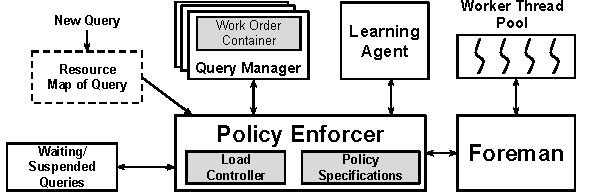
\includegraphics[width=\columnwidth]{figures/Scheduler-Architecture.pdf}
	\vspace*{-1.5em}
	\caption{Overview of the scheduler}
	\label{fig:scheduler-architecture}
	\vspace*{-1.5em}
\end{figure}

An important component of the system is the \textit{Policy Enforcer}.
It selects a query among all the concurrent queries, and schedules its work order for execution. 
This in essence is \textit{a scheduling decision}, and is taken based on a high-level policy provided to the system.
The policy is described in \textit{Policy Specifications}, which is an
abstraction that governs how resources are shared among concurrent queries. 

Policy Enforcer (PE) and various Query Managers (QM) communicate with each other as follows:
\textbf{QM}$\rightarrow$\textbf{PE}: Provides work orders that belong to the managed query for dispatching (to get executed).
\textbf{PE}$\rightarrow$\textbf{QM}: Upon completion of a work order, send a signal so that the QM can then decide if new nodes in the DAG can be activated, and if existing nodes can be marked as completed.
A detailed description of the Policy Enforcer is present in Section~\ref{ssec:policy-enforcer}. 

The Policy Enforcer contains a \textit{Load Controller} module, which is
responsible for ensuring that the system has enough resources to meet the
demands.
A new query in the system presents its resource requirements for its lifetime in the form of a \textit{Resource Map} to the Load Controller.
%The estimates provided in the Resource Map can come from the query optimizer or some other mechanism, which is irrelevant to the scheduler.
A sample resource map is presented in~\cite{supplement}.

The Load Controller determines the fate of a new query. 
If enough resources are available, it admits the query.
If the system risks thrashing due to the admission of the new query, it can take a number of decisions, including wait-listing the query or suspending older active queries to free up resources for the new query.
%The Policy Enforcer maintains queues for wait-listed and suspended queries as shown in Figure~\ref{fig:scheduler-architecture}.
We describe the Load Controller in Section~\ref{ssec:load-control-mech}.

The Policy Enforcer works with another module called the \textit{Learning Agent}. 
Execution statistics of completed work orders are passed from the Policy Enforcer to the Learning Agent.
This component uses a simple learning-based method to predict the time to 
complete future work orders using the execution times of finished work orders. 
Such predictions form the basis for the Policy Enforcer's decisions regarding scheduling the next set of work orders (cf. Section~\ref{ssec:learning} for details on Learning Agent).

%Work orders that are ready to execute are sent to a \textit{Foreman} module. 
%The Foreman simply acts as a link between the overall scheduler and a pool of 
%worker threads. 
The \textit{Foreman} module acts as a link between the Policy Enforcer and a pool of worker threads. 
It receives work orders that are ready for execution from the Policy Enforcer, and dispatches them to the worker threads. 
The Foreman can monitor the number of pending work orders for each worker, and 
use that information for load-balancing when dispatching work orders.
Upon completion of the execution of a work order, a worker sends execution statistics to the Foreman, which are further relayed to the Policy Enforcer.
New work orders due to pipelining are generated similarly (these details are presented in~\cite{supplement}).

\sys{} has two kinds of threads -- a \textit{scheduler} thread and many \textit{worker} threads that perform the actual relational operations as defined by \textit{work orders}. 
More details about the thread model can be found in~\cite{supplement}.

\subsection{Policy Enforcer}\label{ssec:policy-enforcer}
The Policy Enforcer assigns a probability value to each active query in the system. 
A scheduling decision is essentially \textit{probabilistic}, based on these probability values. 
The probability value assigned to a query indicates the likelihood of a work order from that query being scheduled. 
These probability values play a crucial role in the policy enforcement.
In Section~\ref{sec:policy}, we formally derive these probability values for different policies and also establish the relationship between probability values and the policy specifications.

An important information to determine such a probability value is an estimate about the run times of future work orders of the query.
This information provides the Policy Enforcer some idea about the future resource requirements of each query.
As the Policy Enforcer continuously monitors the resource allocation to different queries in the system, using these estimates, it can control the resource allocation with the goal of \textit{enforcing} the specified policy for resource sharing. 
%Using these estimates for the active queries, the Policy Enforcer can control the resource allocation to queries with the goal of \textit{enforcing} the specified policy for resource sharing. 
In the next section, we describe an estimation technique for the execution time of future work orders of a query.
\subsection{Learning Agent}\label{ssec:learning}
The Learning Agent module is responsible for predicting the execution times of the future work orders for a given query. 
It gathers the history of executed work orders of a query and applies a prediction model on such a history to estimate the execution time of a future work order.
This predicted execution time is used to compute the probability assigned to each query (cf. Section~\ref{sec:policy} for probability derivations).

An alternative to the Learning Agent could be a static method that assigns fixed probability values to active queries in the system. 
We now justify the need for the Learning Agent and highlight the limitations of the alternative mentioned above.
An illustrative example is presented in~\cite{supplement}.

The time per work order metric doesn't stay the same throughout a query's lifetime, for reasons such as variations in input data (e.g. skew), CPU characteristics of different relational operators (e.g. scan vs hash probe).
In each phase of the query, the time per work order is different.
As the query plan gets bigger, the number of phases in the plan increase.
In addition, different queries may be in different phases at a given point in time.
To make things more complicated, queries can enter or leave the system at any time.

Therefore, it is difficult to statically pick a proportion of CPU to allocate to the concurrent queries. 
Hence there is a need to ``learn'' the various phases in the query execution and dynamically change the proportion of resources that are allocated to each query, based on each query's phase.
Next, we study the methodology used by the Learning Agent.
\subsubsection{Learning Agent Methodology}
%The Learning Agent builds each query's \textit{execution profile} based 
%on the execution statistics of recently completed work orders for that query.
The Learning agent uses the execution times of previously executed work orders 
($t_{w_{1}}, t_{w_{2}}, \ldots, t_{w_{k}}$) to predict the execution time of 
the next work order ($t_{w_{k+1}}$) for a given query.\footnote{In the beginning of a query execution, when enough information about work order execution times is not available, we use the default probabilities in the Policy Enforcer, instead of using default predicted times in the Learning Agent.}
Figure~\ref{fig:scheduler-cycle} shows the Learning Agent's interaction with the other scheduler components.
%It receives the execution statistics of an  executed work order, and uses this information 
%to predict the execution time of the future work orders. 

\begin{figure}[]
	\centering
	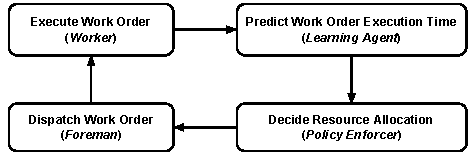
\includegraphics[width=\linewidth]{figures/Compact-SchedulerCycle.pdf}
	\vspace{-1.5em}
	\caption{Interactions among scheduler components}
	\label{fig:scheduler-cycle}
	\vspace{-1.5em}
\end{figure}

The set of previously executed work orders can belong to multiple relational operators in the query operator DAG. 
The Learning Agent stores the execution times of the work orders grouped by their source relational operator, e.g. the execution statistics of select work orders are maintained together and kept separate from those of aggregation work orders. 

%A prediction model is used to estimate the execution time of future work orders. 
\sys{}'s scheduler currently uses linear regression as the prediction model.
We chose linear regression as it is fast, accurate, and efficient w.r.t. the computational and the storage requirements of the model. 
%(New models can be easily added using an abstraction mechanism.) 
More details about our use of linear regression is described in~\cite{supplement}.

The problem of estimating the query execution time is well-studied, but requires complex methods~\cite{duggan2011performance, wu2013towards, li2012gslpi, 
chaudhuri2004estimating}. 
The Learning Agent does not require such methods. 
However, it can combine estimates from other methods with its own estimates.
%i.e. we try to predict the execution times of immediate work orders, as opposed  to a 
%global
%level estimation that may involve estimation of the progress of the query and prediction
%of query/workload completion times. The Learning Agent can be extended to use
%other techniques for the prediction, and is complimentary to other methods for
%estimation.